\documentclass[11pt,conference]{IEEEtran}

\usepackage{amsmath,amssymb,amsfonts}
\usepackage{algorithmic}
\usepackage{array,booktabs}
\usepackage{amsthm}
\usepackage{graphicx}
\usepackage{subcaption}
\usepackage{textcomp}
\usepackage{xcolor}
\usepackage[inline]{enumitem}
\newlist{inlist}{enumerate*}{1}
\setlist[inlist]{label= (\alph*)}
\usepackage{mathpartir,semantic}
\usepackage[colorlinks]{hyperref}
\hypersetup{%
    colorlinks=true,
    linkcolor=blue,
    urlcolor=cyan,
    citecolor=blue
}
\usepackage[style=ieee]{biblatex}
\addbibresource{sources.bib}

\newcommand{\matlab}{MATLAB}
\newcommand{\mmatlab}{\textmu\matlab}
\newcommand{\colorlib}{CoLoR}
\renewcommand{\algorithmiccomment}[1]{\% #1}
\newcommand{\inputcoq}[1]{\InputIfFileExists{#1.v_tex}{}{\typeout{No file #1.v_tex.}}}
\newcommand{\var}[1]{\mathit{#1}}
\newcommand{\func}[1]{\mathsf{#1}}
\newcommand{\iname}[1]{\textsf{#1}}

\theoremstyle{plain} % default
\newtheorem{thm}{Theorem}[section]
\newtheorem{lem}[thm]{Lemma}
\newtheorem{prop}[thm]{Property}
\newtheorem*{cor}{Corollary}

\theoremstyle{definition}
\newtheorem{defn}{Definition}[section]
\newtheorem{example}{Example}[section]
\newtheorem{exercise}{Exercise}[section]
\newtheorem*{prob}{Problem}

\theoremstyle{remark}
\newtheorem*{rem}{Remark}
\newtheorem*{note}{Note}
\newtheorem{case}{Case}

\begin{document}

\title{Final paper: Towards Proving Termination of \texttt{zelda-mosaic} Algorithms under Conditions on the Input}

\author{\IEEEauthorblockN{Justin Do}
\IEEEauthorblockA{\textit{Computer Science} \\
\textit{UNC Chapel Hill}\\
Chapel Hill, USA \\
\texttt{justindo@cs.unc.edu}}
\and
\IEEEauthorblockN{D. Ben Knoble}
\IEEEauthorblockA{\textit{Computer Science} \\
\textit{UNC Chapel Hill}\\
Chapel Hill, USA \\
\texttt{david3@cs.unc.edu}}
}

\maketitle

\begin{abstract}
    We report on a study of previous set of algorithms that we developed for
    building mosaics, implemented in \matlab\@. In particular, we are interested
    in the formalization of the algorithms and the relevant \matlab\ structures
    in Coq~\cite{Coq} and the termination of these algorithms under appropriate
    to-be-determined conditions. We present details on the algorithms along with
    our motivations for studying them. We then discuss an initial foray into
    related work. Next, we show an updated timeline for our progress. Lastly, we
    briefly identify the major contributions of each author to this proposal.
\end{abstract}

% \begin{IEEEkeywords}
% \end{IEEEkeywords}

\section{Summary of Proposal}

We have previously developed \texttt{zelda-mosaic}~\cite{zelda_mosaic} which
includes \matlab~\cite{matlab} code to create tiled ``mosaics'' from a set of
smaller input images. In our original proposal, we set out to prove the
termination of our mosaic-generation algorithms.

In the original work, we took a series of related images (specifically, from one
of the many ``Legend of Zelda'' ({\copyright} Nintendo) games) and automatically
stitched them together to form mosaics of game-related artwork.
\figurename~\ref{F:zelda-mosaic-sample} showcases an example output. The program
is extendable and has been successfully used on several different sizes of
inputs and for applications beyond the original project.

\begin{figure*}[pht]
    \centering
    \begin{subfigure}{0.35\textwidth}
        
\includegraphics[width=\linewidth]{img/oracleofages-original.jpg}
        \caption{Original key-art}
    \end{subfigure}
    \begin{subfigure}{0.35\textwidth}
        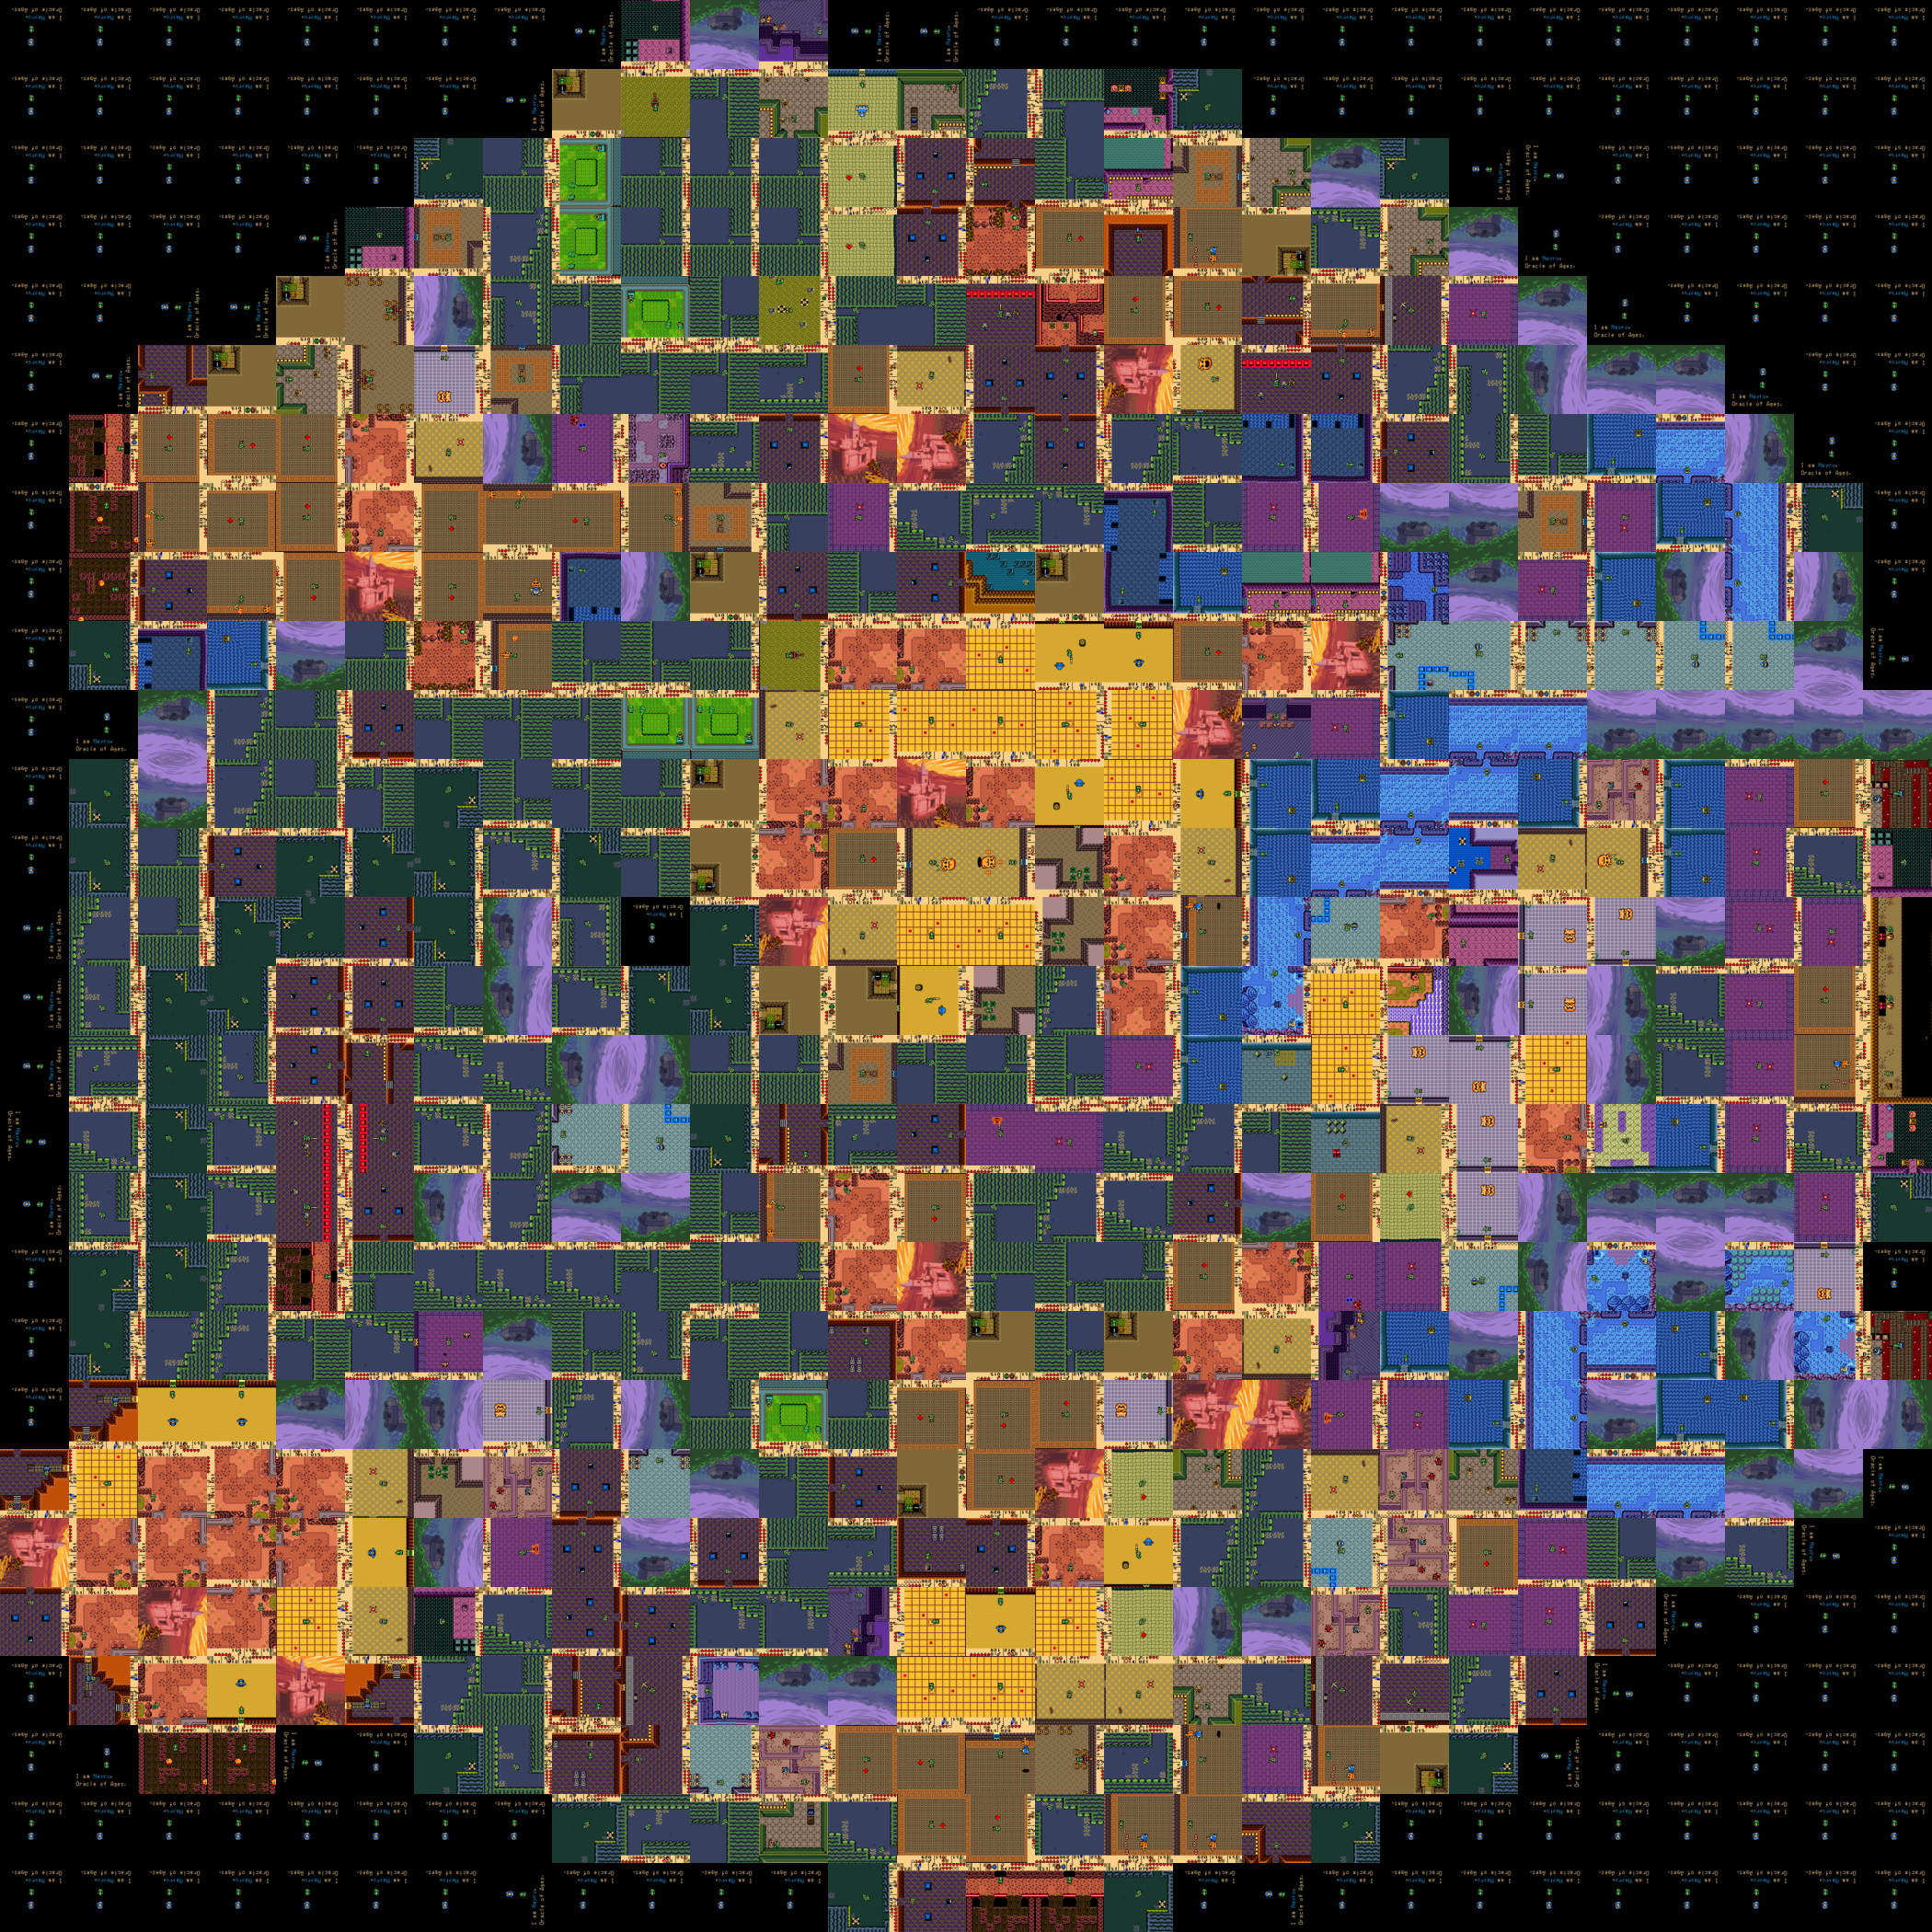
\includegraphics[width=\linewidth]{img/oracle_of_ages_v1.png}
        \caption{Version 1 Mosaic}
    \end{subfigure}
    \begin{subfigure}{0.35\textwidth}
        \includegraphics[width=\linewidth]{img/oracle_of_ages_v2.png}
        \caption{Version 2 Mosaic}
    \end{subfigure}
    \begin{subfigure}{0.35\textwidth}
        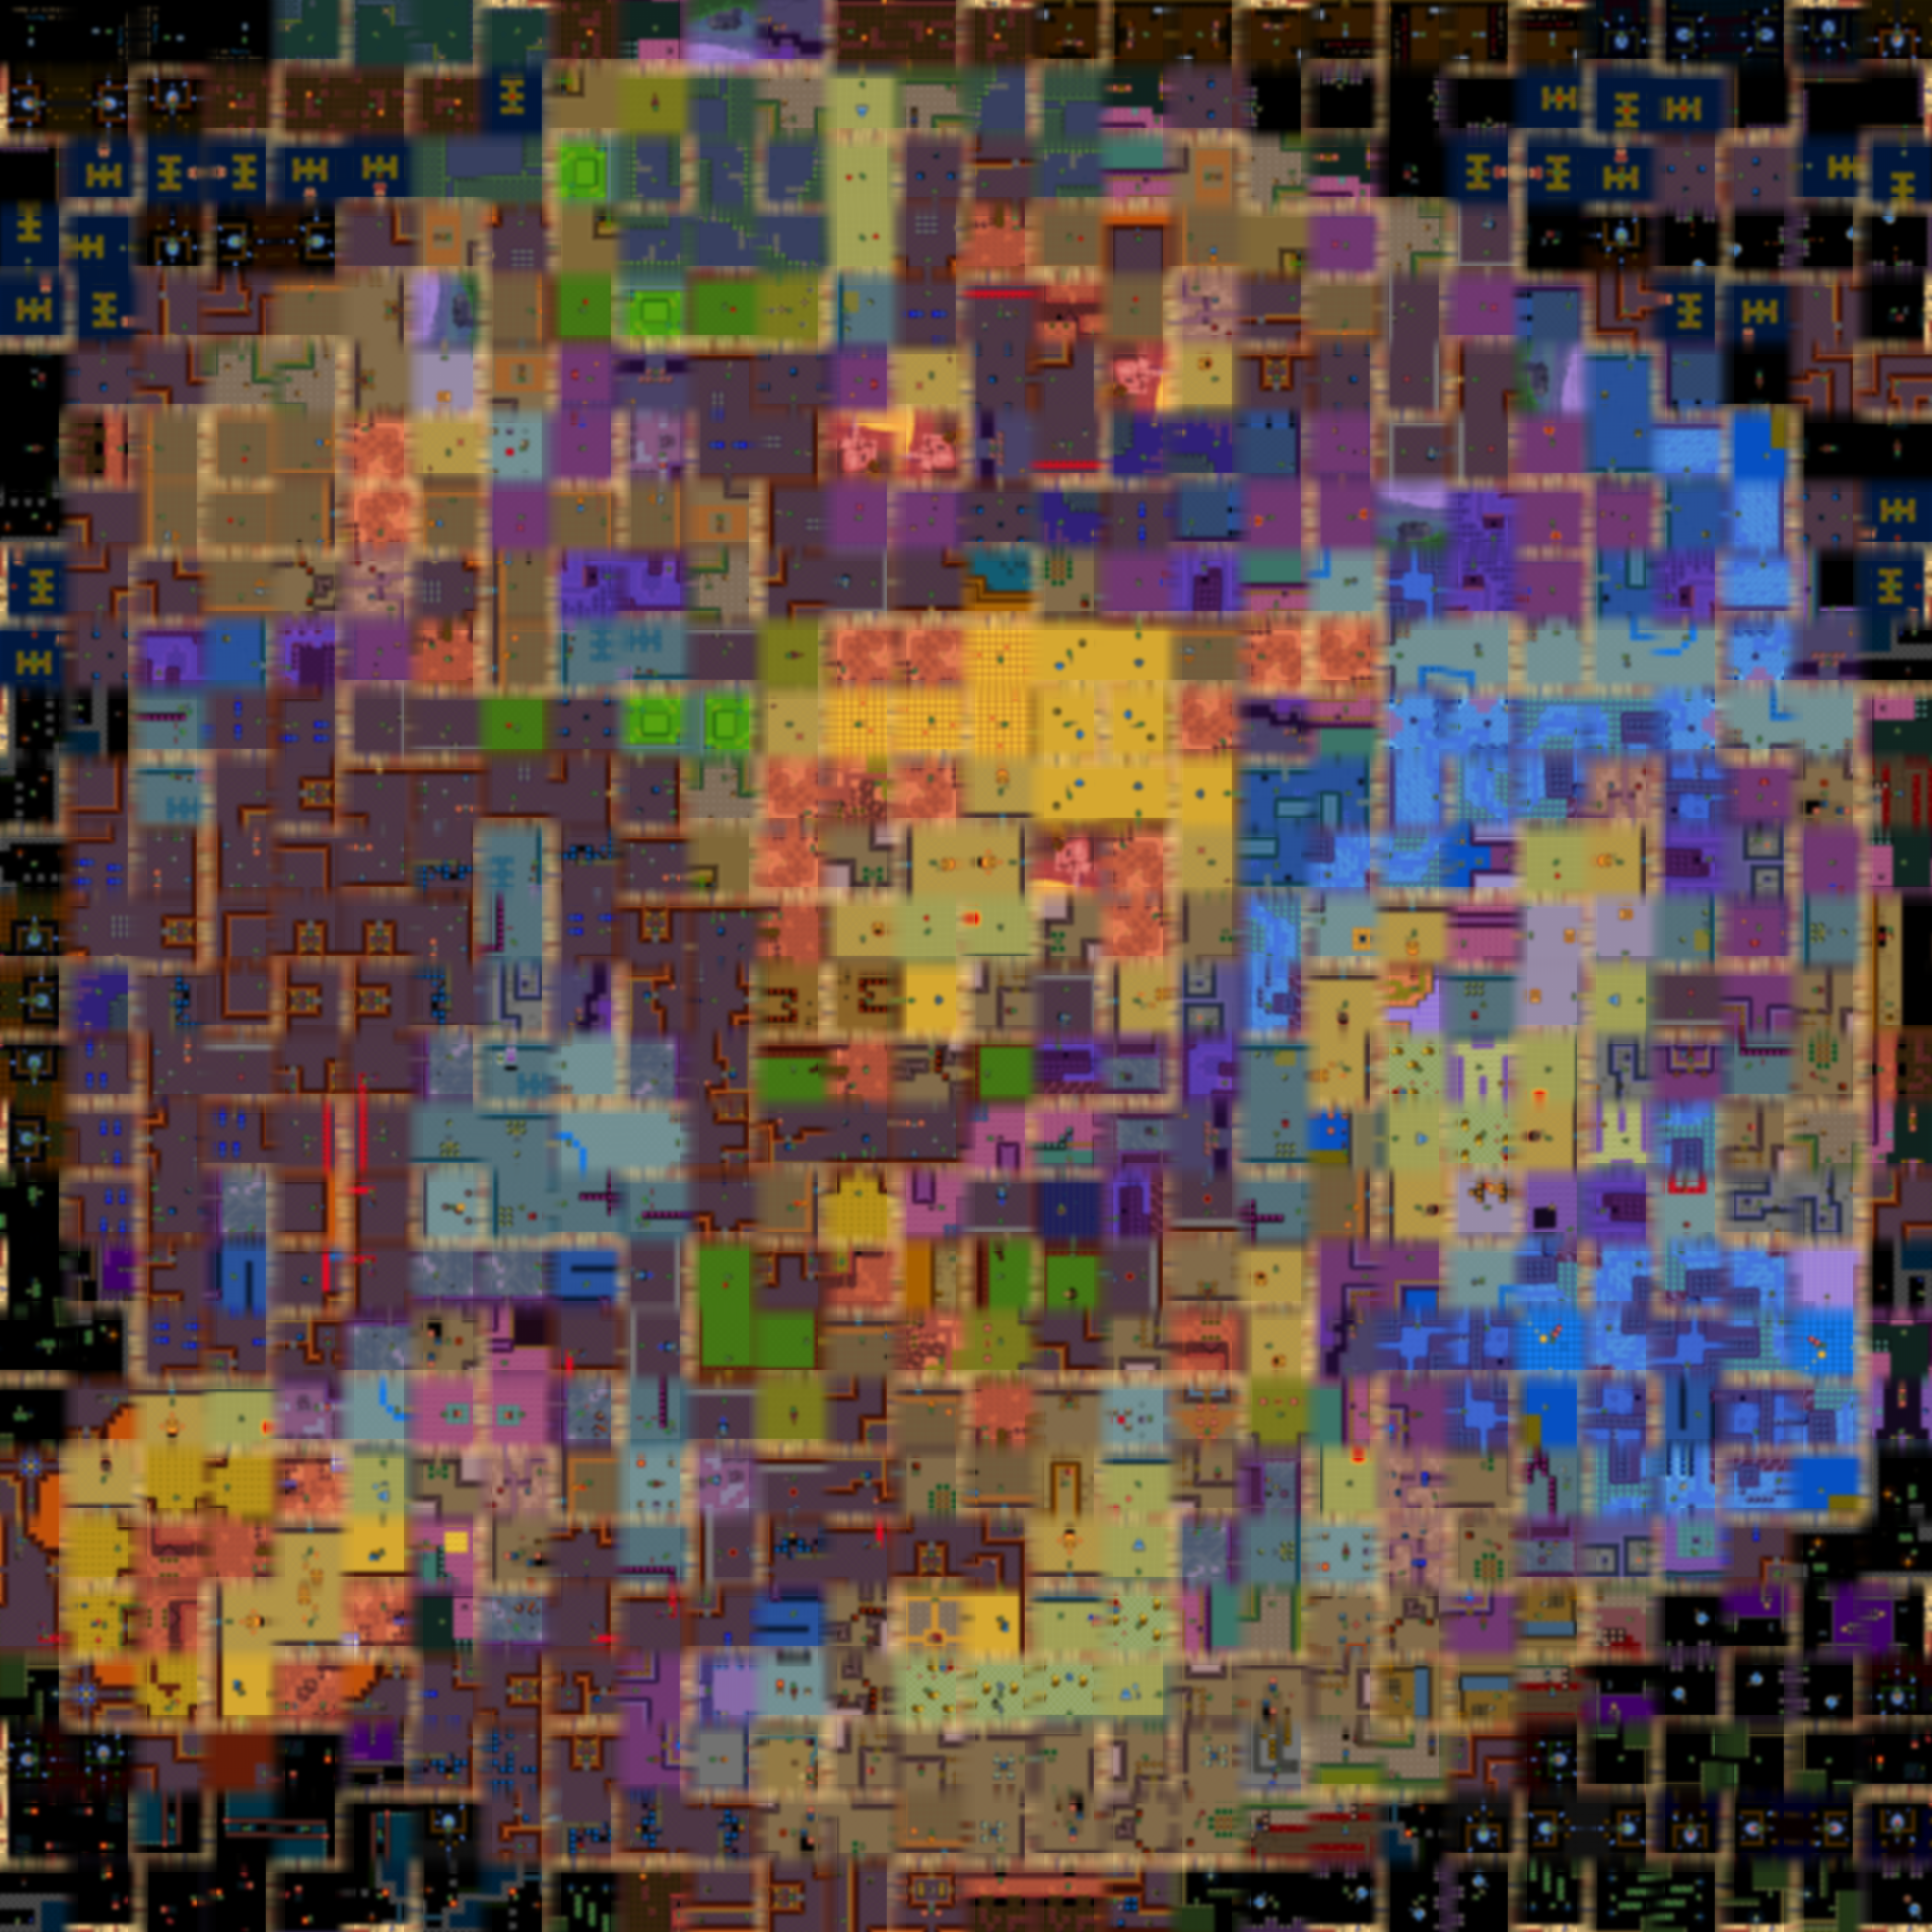
\includegraphics[width=\linewidth]{img/oracle_of_ages_v3.png}
        \caption{Version 3 Mosaic}
    \end{subfigure}
    \begin{subfigure}{0.35\textwidth}
        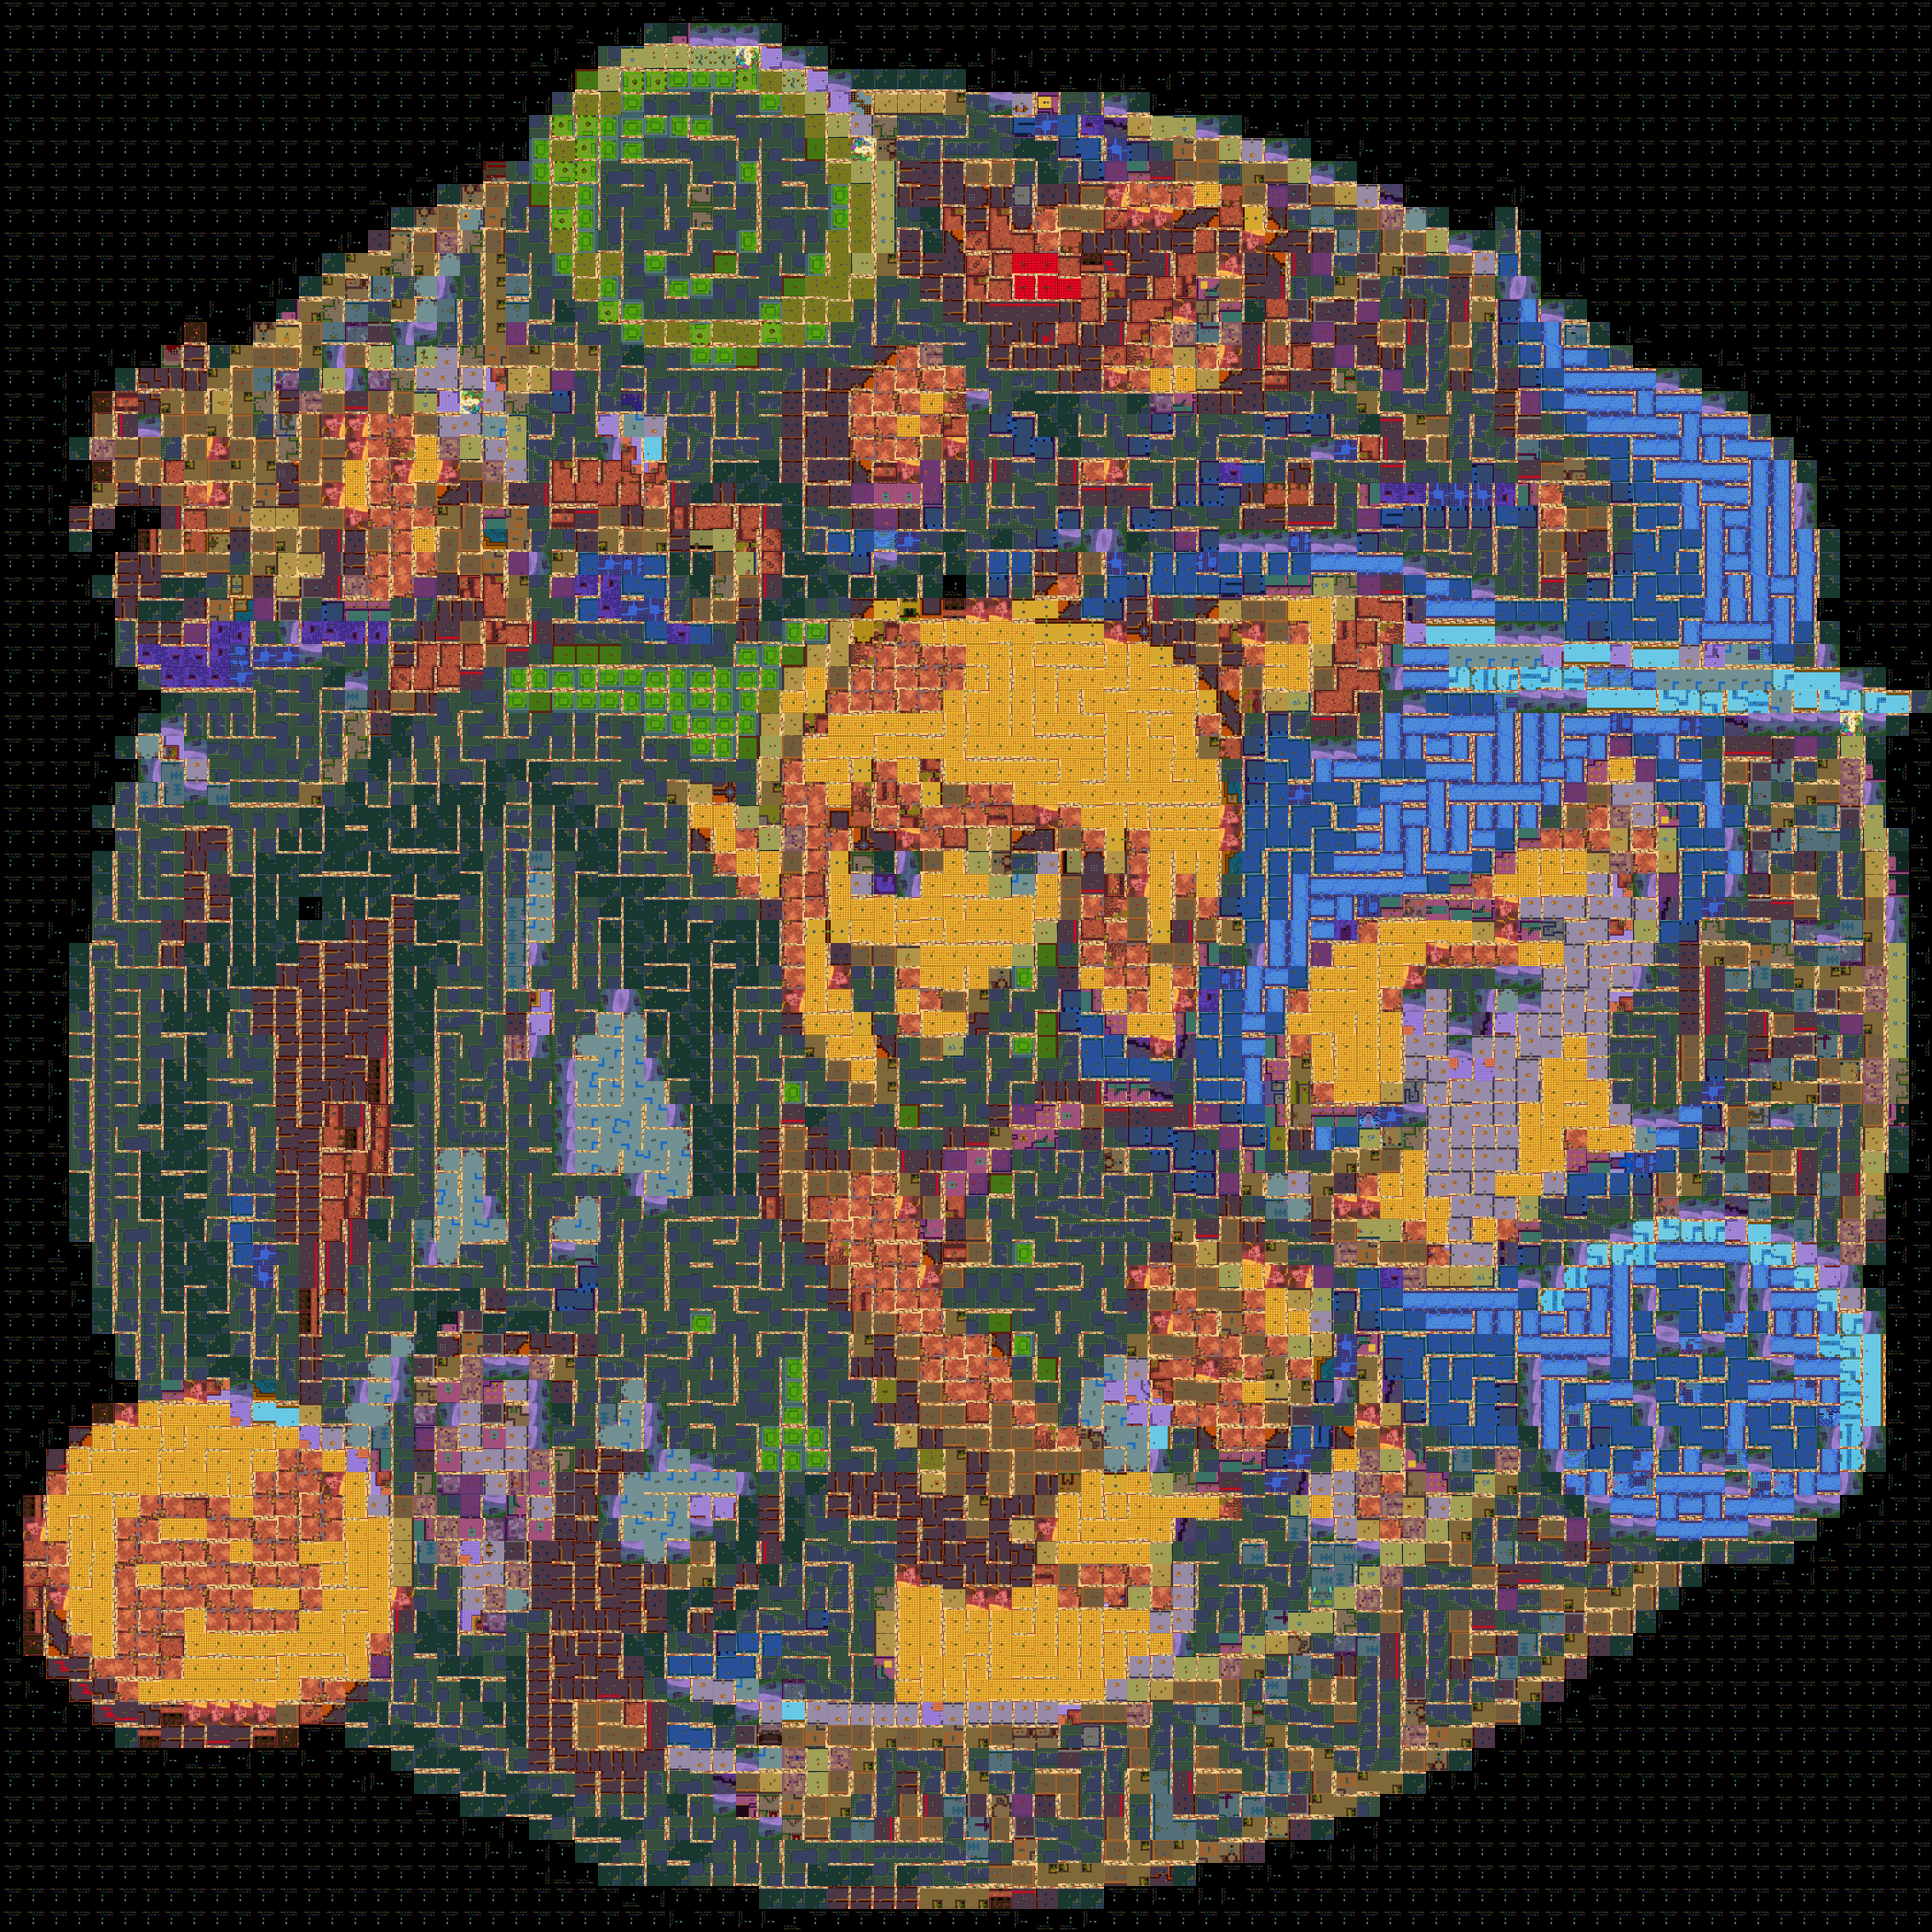
\includegraphics[width=\linewidth]{img/oracle_of_ages_v1_smaller.png}
        \caption{Version 1 Mosaic with smaller inputs}
    \end{subfigure}
    \begin{subfigure}{0.35\textwidth}
        \includegraphics[width=\linewidth]{img/oracle_of_ages_v3_smaller.png}
        \caption{Version 3 Mosaic with smaller inputs}
    \end{subfigure}
    \caption{\texttt{zelda-mosaic} sample}\label{F:zelda-mosaic-sample}
\end{figure*}

We iteratively developed three versions after our initial proof-of-concept. Each
version refines the algorithm of the previous version (for details, the
pseudocode for each algorithm may be found in
\figurename{s}~\ref{alg:v1},~\ref{alg:v2}, and~\ref{alg:v3}). We also further
refined mosaic quality by stitching smaller images, at a performance cost. The
original presentation is publicly available~\cite{zelda_mosaic_pres}, as is a
separate video-recording~\cite{zelda_mosaic_vid}.

Our original goal was to examine these algorithms as implemented in the \matlab\
source and prove, if possible, their termination given well-conditioned input.
With some of the work now behind us, we have a better idea of what this project
entails and how we will be able to reach the finish line.

\section{Progress Report}

The starting point to our project was to fill in some knowledge gaps that we had
not covered in class prior to when we began. Since we planned to model a
program, we needed to know more about the modeling of programs and execution. To
this end, we completed work in \textit{Software Foundations} up to the chapter
\textit{Simple Imperative Programs}~\cite{Pierce:SF1}. This chapter provided
great insight on how to model statements and expressions, maintain state over a
program's execution, and define semantics. After completing this, we were better
able to outline the scope of the project.

Our progress thus far can be divided into two main categories:
\begin{inlist}
\item determining the subset of \matlab\ (dubbed \mmatlab) relevant to our program, and
\item creating data structures and functions suitable to model the behaviors of
    \mmatlab\@.
\end{inlist}

We also identify two main future tasks that will rely upon the completion of
these tasks:
\begin{inlist}
\item binding operations from the \mmatlab\ language to semantics in
    Coq~\cite{Coq}, and
\item using Hoare logic~\cite{Hoare_1969} to prove that the program terminates
    under what pre-conditions.
\end{inlist}

\subsection{\mmatlab}\label{S:mmatlab}

We give a brief overview on \mmatlab, the subset of \matlab\ that we model in
order to prove facts about our programs.

Aside from general programming patterns for control flow, the main syntax of
relevance in our program involves array/matrix accesses and updates, arithmetic
operations, and \matlab-specific primitives such as ranges. We have identified
all of the expressions and statements we expect to use and defined them as
inductive types, shown in \figurename~\ref{fig:inductivetypeexp} and
\figurename~\ref{fig:inductivetypestmt}.

\begin{figure}[ht]
    \centering
    \begin{align*}
        \func{exp} \triangleq\;
        & |\; \func{IntLiteral} \\
        & |\; \func{FloatLiteral} \\
        & |\; \func{AddExp} \\
        & |\; \func{MultExp} \\
        & |\; \func{DivExp} \\
        & |\; \func{EqualsExp} \\
        & |\; \func{NotEqualsExp} \\
        & |\; \func{LTEqualsExp} \\
        & |\; \func{Floor} \\
        & |\; \func{VarRefExp} \\
        & |\; \func{RangeExp} \\
        & |\; \func{MatrixLiteral} \\
        & |\; \func{IndexExp} \\
        & |\; \func{SqueezeExpr} \\
        & |\; \func{SizeExpr} \\
        & |\; \func{LengthExpr} \\
        & |\; \func{ProdExpr} \\
        & |\; \func{SumExpr} \\
        & |\; \func{MinExpr} \\
        & |\; \func{MaxExpr} \\
        & |\; \func{PointWiseExpExp} \\
        & |\; \func{ZerosExp} \\
        & |\; \func{OnesExp} \\
        & |\; \func{InfExp} \\
        & |\; \func{FindExp}
    \end{align*}
    \caption{Skeleton of abstract syntax for expressions used in
    \mmatlab\@.}\label{fig:inductivetypeexp}
\end{figure}

\begin{figure}[ht]
    \centering
    \begin{align*}
        \func{statement} \triangleq\;
        & |\; \func{NoOp} \\
        & |\; \func{Error} \\
        & |\; \func{ExprS} \\
        & |\; \func{AssignS} \\
        & |\; \func{IndexedAssignS} \\
        & |\; \func{SeqS} \\
        & |\; \func{WhileS} \\
        & |\; \func{IfThenElseS} \\
    \end{align*}
    \caption{Skeleton of abstract syntax for statements used in
    \mmatlab\@.}\label{fig:inductivetypestmt}
\end{figure}

Much of the abstract syntax is relatively self-explanatory, so complete
definitions are elided here. However, we wish to draw attention to some of the
less apparent and more interesting syntax present in \mmatlab\@:

\begin{itemize}

    \item \textsf{AddExp}: While this is nominally a regular addition operator,
        \matlab's addition is interesting in that it has overloaded parameter
        types and expected behavior for each. The addition of two numbers is a
        number and the addition of two matrices results in element-wise
        addition, as one might expect. However, the sum of a number and a
        matrix, is a matrix with all elements incremented by the number. Similar
        behaviors hold for \textsf{MultExp} and \textsf{DivExp}.

    \item \textsf{RangeExp}: Like Python, \matlab\ has an expression where a
        starting number and stopping number may be provided, generating an
        inclusive list of all numbers between them.

    \item \textsf{SqueezeExpr}: For multi-dimensional arrays, sometimes the size
        of a particular dimension will be 1. \texttt{squeeze} is a function that
        reduces dimensionality by discarding or ``squeezing'' these superfluous
        dimensions.

\end{itemize}

\subsection{Data Structures and Functions}

Our program is used for image processing; thus, many computations are made on
images, which are represented as arrays in \matlab\@. Additionally, we deal with
matrices of images, so we need to model multi-dimensional matrices. Since
multi-dimensional matrices can have arbitrarily many dimensions, we decided the
best abstraction for this in Coq would be built on top of the \textsf{Vector}
type which was originally implemented in the \colorlib\
library~\cite{BLANQUI_2011} and eventually ported to the Coq standard library.
In Coq, \textsf{Vector} is a dependent type~\cite{Bove2009,Thorsten_2010}; the
number of elements in a \textsf{Vector} is part of its type, written
\texttt{Vector.t A n} for a vector containing \(n\) elements of type \(A\).
Since \textsf{Vector}s are polymorphic, we noted that a \textsf{Vector} could
contain \textsf{Vector}s provided they are all the same type (which includes
length, as noted). That is, we can stack \textsf{Vector}s to form, \emph{e.g.},
\texttt{Vector.t (Vector.t A m) n}. From there, we defined a type-constructor
\textsf{Matrix} taking a list of dimensions, which represents a \textsf{Vector}
of \textsf{Vector}s. It can be used as the type of an arbitrary
\(n\)-dimensional matrix containing elements of type \(A\).

Due to the implementation of \textsf{Vector} in the Coq standard library, we
needed to greatly extend the functionality of our \textsf{Matrix} type. To that
end, we have begun implementing \textsf{Matrix} functions such as element
access, which is non-trivial for matrices with an arbitrary number of
dimensions\footnote{In particular because of the dependent types; see also
\url{https://stackoverflow.com/q/66863226/4400820}}. Additionally, the existing
implementation of element access in Coq's \textsf{Vector} type uses the
unfamiliar \textsf{Fin} type, an abstraction for carrying proofs that a
particular number belongs to finite range of numbers. In order to access an
element of a \textsf{Vector}, one must supply such a proof; for our purposes, we
use \texttt{Fin.of\_nat}, which gives either such a proof or a witness that the
number is outside the range. This behavior is captured by the \textsf{sumbool}
built-in, which required further research on our behalf. Given the number of
ways that matrices can be indexed in \matlab\ and the complexity introduced by
Coq's implementation of \textsf{Vector}s, we see this as the main bottleneck for
our progress. We still need to implement many \textsf{Matrix} operations, such
as accesses over ranges and over an entire dimension.

\subsection{Binding Operations and Semantics}

While we have not yet bound any of our functions or data types to the statements
or expressions in \S~\ref{S:mmatlab}, we have naturally been thinking about them
throughout the whole process. The functions we write are intended to implement
the evaluation of the corresponding expressions. In the style of
\texttt{Imp}~\cite{Pierce:SF1}, we intend to write a deterministic expression
evaluation function; we will then provide semantics for program execution.
Execution cannot be defined as a function in Coq because it may be
non-terminating. We have had to consider what operations are be allowed and
whether checks for undesired behavior (\emph{e.g.}, dynamic type mismatches)
should be implemented in the underlying functions or in a semantic check.

\subsection{Hoare Logic}

We have a significant amount of work to do in modeling \mmatlab, but the
blue-sky goal remains to prove the termination of our program given that certain
preconditions hold. Ben has been studying Hoare logic~\cite{Hoare_1969}, the
relevant background material for this problem, as part of his Thesis
requirement. What will be possible to prove will be determined in part by what
we are able to successfully model, given the time constraints. However, as a
preliminary step, we have studied partial Hoare logic and total Hoare logic to
provide more context for the task ahead of us. In this exploration, we found
that partial Hoare logic is a weak statement about programs; namely, given
preconditions \(P\) and postconditions \(Q\) and a program \(C\), the Hoare
triple \(\{P\}C\{Q\}\) asserts that \emph{if} \(C\) terminates, then the
pre-conditions imply the post-conditions. Total Hoare logic, by contrast, is a
stronger version of this claim: \(C\) is asserted to terminate. Thus a proof in
total Hoare logic necessitates a proof that \(C\) terminates; the inference
rules are accordingly adjusted. The primary adjustment is to the rule for while
loops, which are guaranteed to terminate by relation to a decreasing sequence
(with respect to a well-founded order). Given that we are trying to prove
termination, it seems likely that we will need to use total Hoare logic in the
relevant proofs.

\begin{figure}[ht]
    \textbf{Input}: image \(key\_art\), images \(thumbnails\), integer \(size\) \\
    \textbf{Output}: image \(tiles\)
    \begin{algorithmic}
        \STATE{\(tiles \gets \textrm{MAT2TILES}(key\_art, size, size)\)}
        \FOR{\(tile \in tiles\)}
            \FOR{\(thumbnail, i \in thumbnails, [1..|thumbnails|]\)}
                \STATE{\(mses_i \gets \textrm{immse}(tile, thumbnail)\)}
            \ENDFOR
            \STATE{\(best\_indices \gets \textrm{find} (mses = \min mses)\)}
            \STATE{\(best\_index \gets best\_indices_0\)}
            \STATE{\(tile \gets thumbnails_{best\_index}\)}
        \ENDFOR
    \RETURN{\(tiles\)}
    \end{algorithmic}
    \caption{Algorithm: Version 1}\label{alg:v1}
\end{figure}

\begin{figure}[ht]
    \textbf{Input}: image \(key\_art\), images \(thumbnails\), integer \(size\) \\
    \textbf{Output}: image \(tiles\)
    \begin{algorithmic}
        \STATE{\(tiles \gets \textrm{MAT2TILES}(key\_art, size, size)\)}
        \STATE{\(used \gets \emptyset\)}
        \STATE{\(threshold \gets 1\)}
        \IF{\(|thumbnails| < |tiles|\)}
            \STATE{\(threshold \gets \lceil{|tiles| / |thumbnails|}\rceil\)}
        \ENDIF
        \FOR{\(tile \in tiles\)}
            \FOR{\(thumbnail, i \in thumbnails, [1..|thumbnails|]\)}
                \STATE{\(mses_i \gets \textrm{immse}(tile, thumbnail)\)}
            \ENDFOR
            \STATE{\(best\_indices \gets \textrm{find} (mses = \min mses)\)}
            \STATE{\(best\_index \gets best\_indices_0\)}
            \WHILE{\(used_{best\_index} \ge threshold\)}
                \STATE{\(mses_{best\_index} \gets \infty\)}
                \STATE{\(best\_indices \gets \textrm{find} (mses = \min mses)\)}
                \STATE{\(best\_index \gets best\_indices_0\)}
            \ENDWHILE
            \STATE{increment \(used_{best\_index}\)}
            \STATE{\(tile \gets thumbnails_{best\_index}\)}
        \ENDFOR
        \RETURN{\(tiles\)}
    \end{algorithmic}
    \caption{Algorithm: Version 2}\label{alg:v2}
\end{figure}

\begin{figure}[ht]
    \textbf{Input}: image \(key\_art\), images \(thumbnails\), integer \(size\) \\
    \textbf{Output}: image \(tiles\)
    \begin{algorithmic}
        \STATE{}\COMMENT{Repeat Version 2}
        \STATE{\(tiles \gets \textrm{Version2}(key\_art, thumbnails, size)\)}
        \STATE{\(tiles \gets \textrm{imgaussfilt}(tiles)\)}
        \STATE{\(strip\_size \gets \lfloor{size / 8}\rfloor\)}
        \STATE{}\COMMENT{Blur by averaging}
        \FOR{horizontal \(strip \in tiles\)}
            \STATE{\(strip \gets \textrm{mean}({strip})\)}
        \ENDFOR
        \FOR{vertical \(strip \in tiles\)}
            \STATE{\(strip \gets \textrm{mean}({strip})\)}
        \ENDFOR
        \RETURN{\(tiles\)}
    \end{algorithmic}
    \caption{Algorithm: Version 3}\label{alg:v3}
\end{figure}

\section{Results}\label{S:results}

In this section, we present the results of our work towards proving termination
of our mosaic algorithm. As noted, our primary accomplishment is the definition
of a workable matrix type and operations on it. This matrix type is intended to
support the operations needed to implement expression evaluation for \mmatlab, a
crucial component of implementing the language's semantics. It remains to finish
implementing expression evaluation and the necessary matrix operations, to give
operation semantics for the statements of \mmatlab, to give a total Hoare logic
for the language, and then finally to give the proofs of termination of the
algorithms found in \figurename{s}~\ref{alg:v1},~\ref{alg:v2}, and~\ref{alg:v3}.

We present, in order,
\begin{inlist}
\item the Coq definition of the polymorphic matrix type \texttt{matrix A} and
    corresponding operations;
\item key theorems and sketches of their proofs about the matrix type and its
    operations; and
\item advanced tactics, automation, and ideas for Coq proofs used in the
    development.
\end{inlist}

% TODO: update zelda_mosaic_proof version with final commit

All code may be found at the project repository~\cite{zelda_mosaic_proof}. Most
of the work in this section corresponds to the file \texttt{Lib Matrix.v}.

\subsection{Defining Matrices}\label{S:matrix_defn}

First, we define the matrix type. After noting that it allows invalid matrices
to be formed, we define the well-formed property on matrices in two equivalent
ways. Finally, we give an overview of the Coq definitions of three operations on
matrices: computing their shape, linearizing, and linear indexing. We briefly
mention the beginning of our work on multi-dimensional and range-based indexing.

\subsubsection{The matrix type}

As mentioned in \S~\ref{S:design_dependent}, our original formulation of
matrices as nested dependent \texttt{Vector.t}s quickly grew in complexity.
We abandoned that approach in favor of a type that is not guaranteed to behave
well, but whose definition makes defining operations more
natural~\cite{SO_2021_2}. This approach removes the proofs that dependent types
provide automatically, so we have to give those ourselves.

The new design pairs the dimensionality of a matrix, called its \emph{shape},
with its \emph{contents}. The pairing is done via \emph{Record} types (see the
Coq manual~\cite{Coq}), which are tuples with named elements. The definition
follows below:

\begin{align*}
    & \func{matrix} (\var{A}: \var{Type}) \triangleq \\
    & \{
        \func{shape}: \func{list}\, \mathbb{N},
        \func{contents}: \func{matrix\_content}\, \var{A}
    \}
\end{align*}

The shape is a list of naturals. Each natural corresponds (in a well-formed
matrix) to the number of elements of the matrix in that dimension. For example,
a vector of five (5) elements has shape \texttt{[5]}, while a two-dimensional
matrix of three-by-two elements has shape \texttt{[3; 2]}. The vacuous case,
when the shape is the empty list, is a single scalar value: there is no matrix.

In parallel, the contents are wrapped in an inductive polymorphic type
\(\func{matrix\_content}\, \var{A}\). The type's two constructors correspond to
the two cases above: a \(\func{Matrix}\) contains a list of
\(\func{matrix\_content}\, \var{A}\) values. The \(\func{Matrix}\) constructor,
in a well-formed matrix, corresponds to one dimension of the shape. A
\(\func{Scalar}\) contains exactly a value of type \(\var{A}\) and is the
conceptually the base-case for the matrix type.

\begin{align*}
    & \func{matrix\_content} (\var{A}: \var{Type}) \triangleq\; \\
    & |\; \func{Scalar}: \var{A} \to \func{matrix\_content}\, \var{A} \\
    & |\; \func{Matrix}: \func{list}\, (\func{matrix\_content}\, \var{A}) \to \func{matrix\_content}\, \var{A}
\end{align*}

We provide a few concrete examples of mathematical objects in the space of
scalars and multi-dimensional matrices containing a single type of object in
Table~\ref{T:matrices}. Each example shows standard mathematical notation, the
Coq notation using our matrix type, and the resulting type of the value in Coq.

\begin{table*}[ht]
    \centering
    \begin{tabular}{c >{\ttfamily}c >{\ttfamily}c}
        Mathematical notation & Coq notation & Coq type \\ \toprule
        \(5\) & \{| shape := []; contents := Scalar 5 |\} & matrix nat \\
        \(\begin{bmatrix}
            1 & 2 & 3
        \end{bmatrix}\)
        & \{| shape := [3]; contents := Matrix [Scalar 1; Scalar 2; Scalar 3] |\} & matrix nat \\
        \\
        \(\begin{bmatrix}
            1 & 2 \\
            3 & 4 \\
            5 & 6
        \end{bmatrix}\)
        & \{| shape := [3; 2]; contents := Matrix [
        & matrix nat \\
        & Matrix [Scalar 1; Scalar 2]; & \\
        & Matrix [Scalar 3; Scalar 4]; & \\
        & Matrix [Scalar 5; Scalar 6]] |\} &
    \end{tabular}
    \caption{Example matrices and their Coq equivalents}\label{T:matrices}
\end{table*}

\subsubsection{The well-formed property}

As suggested above, the lack of dependent typing means a value of type
\(\func{matrix}\, \var{A}\) is \emph{not} guaranteed to be well-formed. All of
the following are valid but nonsensical values:

\begin{verbatim}
{| shape := [];
   contents := Matrix [Scalar 1] |}
{| shape := [2];
   contents = Matrix [Scalar 2] |}
{| shape := [1; 2; 3; 0];
   contents = Scalar 0 |}
\end{verbatim}

In the first case, we have a matrix with no dimensions, which should be a scalar
and is not. In the second case, we have a one-dimensional matrix of two
elements which only contains one element. In the third, we have an empty
four-dimensional matrix which is actually a scalar. None of these pairings makes
sense---we need a way to exclude them from our results, effectively categorizing
these matrices as ``not well-formed.'' Conversely, we would like a way to
categorize matrices as well-formed.

We have informally given pieces of the definition in laying our the relationship
between shape and contents; here, we make the definition more precise. A matrix
is well-formed if, and only if,
\begin{itemize}
    \item the shape is an empty list, and the contents are a single scalar value;
        or
    \item the shape is a non-empty list consisting of a head \(n\) representing
        the length of the first dimension and tail \(t\) representing the shape
        of the subsequent dimensions, and the contents is a \(\func{Matrix}\)
        containing a list with length \(n\), and each element of the list is
        well-formed with respect to \(t\).
\end{itemize}
In Coq, we express this definition via a recursive definition
\(\func{well\_formed'}\) which computes a proposition, or proof-burden, over a
shape and contents. We wrap this up in a definition \(\func{well\_formed}\),
which unpacks a matrix for use with \(\func{well\_formed'}\). With this
definition, we can theorems in terms of matrices that are assumed to be
well-formed or that must be shown to be well-formed.

In the course of our development, we discovered that this computational version
did not always provide a convenient means to work a proof. Clearly, the
recursive nature of matrices and well-formedness means that most proofs will be
by induction. But induction on what? There is no induction principle for the
record type, so we must choose from induction on the shape or on the contents.
It turns out that there is a natural inductive version of the well-formed
property that permits induction on evidence. In \S~\ref{S:matrix_thm} we will
state and sketch the equivalence theorem between the two definitions. For now,
we give the judgment rules for \(\func{well\_formedI'}\), the inductive
counterpart to \(\func{well\_formed'}\) in \figurename~\ref{F:wfI}. We wrap the
inductive proposition in \(\func{well\_formedI}\), which unpacks a matrix the
same way as \(\func{well\_formed}\).

\begin{figure*}[ht]
    \centering
    \begin{mathpar}
        \inference[\iname{WF\_Scalar}]{%
            a: A
        }{\func{well\_formedI'}\, []\, (\func{Scalar}\, a)}

        \and

        \inference[\iname{WF\_Empty}]{%
            t: \func{list}\, \mathbb{N}
        }{\func{well\_formedI'}\, (0::t)\, (\func{Matrix}\, [])}

        \and

        \inference[\iname{WF\_Cons}]{%
            h: \mathbb{N} &
            t: \func{list}\, \mathbb{N} &
            m: \func{matrix\_contents}\, \var{A} \\
            ms: \func{list}\, (\func{matrix\_content}\, \var{A}) &
            \func{well\_formedI'}\, (h::t)\, (\func{Matrix}\, ms) &
            \func{well\_formedI'}\, t\, m
        }{\func{well\_formedI'}\, (1+h::t)\, (\func{Matrix}\, (m::ms))}

    \end{mathpar}
    \caption{Inductive judgments for the well-formed property of
    matrices}\label{F:wfI}
\end{figure*}

The important features of the judgements are \(\iname{WF\_Empty}\) and
\(\iname{WF\_Cons}\). The judgement \(\iname{WF\_Empty}\) corresponds to the
vacuous case: all elements in an empty list are well-formed with respect to any
shape (there are no such elements!). The judgment \(\iname{WF\_Cons}\) provides
a judgment for increasing the size of the first dimension of a well-formed
matrix by adding a well-formed component to the contents.

It is easy to prove that all the matrices in Table~\ref{T:matrices} are
well-formed with respect to both definitions. It is likewise easy to prove that
the previously-sketched invalid examples are not well-formed under both
definitions.

\subsubsection{Some operations on matrices}

The operations we have defined are computing the shape of a matrix, linearizing
the matrix, and indexing a multi-dimensional matrix linearly. We will discuss
these and give a brief note about our approach to multi-dimensional range-based
indexing.

\paragraph{Computing the shape of a matrix} While each matrix carries its shape
as part of the record pairing, it is occasionally convenient to compute from the
contents alone the shape. There are two subtleties worth mentioning: first, the
computation is only valid for well-formed matrices because it relies on
assumptions about the relationship between different components of the contents.
Second, the computed shape may not be the most general: we have already seen
that, when one dimension in a matrix has shape zero, the subsequent dimensions
can be arbitrarily sized and the result is still well-formed! This impacts the
correctness statement for shape-computation: on a well-formed matrix, it may not
give the exact same shape, yet it will give a shape such that the original
matrix is well-formed with respect to the new shape. We can call this
``normalization'' of the shape, as it discards dimensions that follow a
zero-sized dimension. See \S~\ref{S:matrix_thm} for more details on
normalization via shape computation. The definition is straightforward: the
function \(\func{compute\_shape}\) yields
\begin{itemize}
    \item an empty list when the contents consist of a single scalar;
    \item a singleton list containing zero when the contents consist of an empty
        matrix; and
    \item a list with head the length of the matrix contents and tail the
        computed shape of just one of the contents when the contents
        consist of a non-empty matrix.
\end{itemize}
This last bullet explains why the function is only valid on well-formed
matrices: it implicitly assumes that all the elements of the matrix contents
have the same computed shape, which is only true when the matrix is well-formed.
The same definition is given below:

\begin{align*}
    & \func{compute\_shape}(\var{m}) \triangleq \\
    & \begin{cases}
        [] & m = \func{Scalar}\, a \\
        [0] & m = \func{Matrix}\, [] \\
        |\var{ms}| :: \func{compute\_shape}\, m' & m = \func{Matrix}\, \var{ms}, \\
        & \var{ms} = m'::t
    \end{cases}
\end{align*}

\paragraph{Linearizing a matrix} See \S~\ref{S:design_linearize} for more
details on matrix linearization. To define linearization in Coq, we use a
two-stage unpacking as with other matrix operations. The function
\(\func{linearize'}\) turns scalars into a singleton list and recursively
flat-maps itself over matrices to produce the one-dimensional matrix as a list.
The function \(\func{linearize}\) unpacks a matrix, then transforms the contents
by wrapping the result of mapping \(\func{linearize'}\) into \(\func{Scalar}\)s
in a \(\func{Matrix}\) and transforms the shape by taking the product of the
(normalized) shape of the matrix. Recall that the length of the linearized
vector is the product of the sizes of all the dimensions. The definitions are
spelled out below:

\begin{align*}
    & \func{linearize'}(\var{contents}) \triangleq \\
    & \begin{cases}
        [\var{a}] & \var{contents} = \func{Scalar}\, \var{a} \\
        \func{flat\_map}\, \func{linearize'}\, \var{ms} & \var{contents} =
        \func{Matrix}\, ms
    \end{cases} \\
    & \func{linearize}(\{\var{contents}, \var{shape}\}) \triangleq \\
    & \{ \var{shape} = \left[\prod \func{compute\_shape}\, \var{contents}\right]; \\
    & \ \, \var{contents} = \func{Matrix}\, (\func{map}\, \func{Scalar}\, (\func{linearize'}\, \var{contents})) \}
\end{align*}

\paragraph{Linearly indexing a matrix} Given the operation to linearise a
matrix, one-based linearly indexing is easy. See \S~\ref{S:design_linear_index}
for details on linear indexing. The function \(\func{nth}\) takes a matrix \(m\)
and an index \(n\); it returns the one-based linearly indexed content of \(m\)
at \(n\) (wrapped in the option constructor \(\func{Some}\)) if \(n\) is in
bounds relative to \(m\). When \(n\) is out of bounds, the result is
\(\func{None}\). For one-based indexing with functions that naturally use
zero-based indexing, we use \(n-1\). We should note that the current version of
\(\func{nth}\) has the subtle bug that indexing at \(n=0\) currently returns the
same as indexing at \(n=1\), when it should in fact be out of bounds and thus
\(\func{None}\)---a simple \texttt{if} or \texttt{match} guard would cover this
case.

\subsection{Key Theorems about Matrices}\label{S:matrix_thm}

Unless otherwise stated, the key theorems are predicated on all matrices
involved being well-formed.

The key theorems of our proof development are
\begin{inlist}
\item that the two different definitions of the well-formed property agree
    (Theorem~\ref{Th:well_formed_agree});
\item that \(\func{compute\_shape}\) normalizes by preserving the well-formed
    property (Theorem~\ref{Th:compute_shape_wf_normalizes}); and
\item that \(\func{linearize}\) is correct, \textit{i.e.}, that
    \(\func{linearize'}\) produces a list with size the product of the shape and
    that \(\func{linearize}\) preserves the well-formed property
    (Theorems~\ref{Th:linearize_product} and~\ref{Th:linearize_wf}).
\end{inlist}
We present these, along with a sketch of their proofs, in order.

\begin{thm}[Well-formed definitions agree]\label{Th:well_formed_agree}
    For all matrices \(m\), \(m\) is well-formed under the computational
    definition \(\func{well\_formed}\) if-and-only-if \(m\) is well-formed under
    the inductive definition \(\func{well\_formedI}\). (See
    \texttt{well\_formed\_agree} in the Coq
    development~\cite{zelda_mosaic_proof}.)
\end{thm}

\begin{proof}
    We begin with the forward direction and proceed by induction on the contents
    of \(m\); for each case of the contents, we also consider the cases of the
    shape. Several cases are immediately contradictory, since the resulting
    \(m\) could not have been well-formed in the first place. In the remainder,
    we must prove \(\func{well\_formed}\, m\) implies \(\func{well\_formedI}\,
    m\).

    The base case is easy: simply use \(\iname{WF\_Empty}\).

    In the inductive case, we can use the well-formed hypothesis together with
    the induction hypothesis and auxiliary Lemma~\ref{Lem:wfI_all_wf_t} to
    finish.

    Now the backwards direction. We must prove that \(\func{well\_formedI}\, m\)
    implies \(\func{well\_formed}\, m\). We proceed by induction on the evidence
    for the hypothesis \(\func{well\_formedI}\, m\).

    The base cases are straightforward and follow readily from the definition.

    In the inductive case, we can use the inductive hypotheses to conclude.
\end{proof}

\begin{lem}\label{Lem:wfI_all_wf_t}
    If all elements of the list \(\var{ms}\) are well-formed (using the inductive
    definition) with respect to some shape \(t\), then the following matrix is
    also well-formed: \(\{ \var{shape} = |\var{ms}| :: t; \var{contents} =
    \func{Matrix}\, \var{ms} \}\).
\end{lem}

The proof is straightforward by induction on \(\var{ms}\).

\begin{thm}[Computing the shape normalizes it]\label{Th:compute_shape_wf_normalizes}
    For all matrices \(m\), if \(m\) is well-formed than so is the following
    matrix: \(\{ \var{shape} = \func{compute\_shape}\, m; \var{contents} =
    \func{contents}\, m \}\).
\end{thm}

\begin{proof}
    We proceed by induction on the contents of \(m\); for each case of the
    contents, we also consider the cases of the shape. Several cases are
    immediately contradictory, since the resulting \(m\) could not have been
    well-formed in the first place.

    The base case is straightforward from the definition of
    \(\func{well\_formed}\).

    In the inductive case, we have to deal with a \(\func{Matrix}\) of some list
    \(\var{ms}\). We proceed by case analysis on the list; the empty case is
    easy. When the list is non-empty, we are left to prove the critical
    assumption in the definition of \(\func{compute\_shape}\); namely, that all
    the elements in a well-formed matrix have the same computed shape. This is
    done by application of the induction hypothesis and observing that any
    element in the non-empty \(\var{ms}\) has the same computed shape, thanks to
    Lemma~\ref{Lem:wf_same_shape}.
\end{proof}

\begin{lem}\label{Lem:wf_same_shape}
    Given any two matrices \(m_1, m_2\) that are well-formed with respect to the
    same shape, \(\func{compute\_shape}\, m_1 = \func{compute\_shape}\, m_2\).
\end{lem}

The proof is straightforward by induction on the shape combined with case
analysis on the two matrices.

\begin{thm}[Linearize has resulting shape the product of the original]\label{Th:linearize_product}
\end{thm}

\begin{thm}[Linearize preserves the well-formed property]\label{Th:linearize_wf}
\end{thm}

\subsection{Advanced Coq for Matrices}\label{S:matrix_coq}

{\printbibliography}

\end{document}
